% %-----------------------------------------------------------
% \section{Métricas do projeto}
% % ----------------------------------------------------------
% Visando acompanhar quantitativamente a evolução no desenvolvimento do \gls{ifriends}, a equipe realiza medições mensalmente, que podem ser observadas na \autoref{tabela de métricas}, conforme os itens: arquivos, classes, porcentagem da cobertura dos testes unitários, \textit{commits}, entidades alocadas no banco de dados, interfaces, quantidade de linhas de código, métodos, \textit{posts} do \textit{blog}, quantidade de testes unitários aplicados, requisitos cumpridos, quantidade de reuniões, tamanho da aplicação em \textit{Mega Bytes} e vídeos publicados no canal do \gls{youtube}. Vale lembrar que os valores inseridos serão contados acumulativamente. 

% \begin{figure}[htb]
% \centering
% \caption{Tabela de métricas}
% \label{tabela de métricas}
% 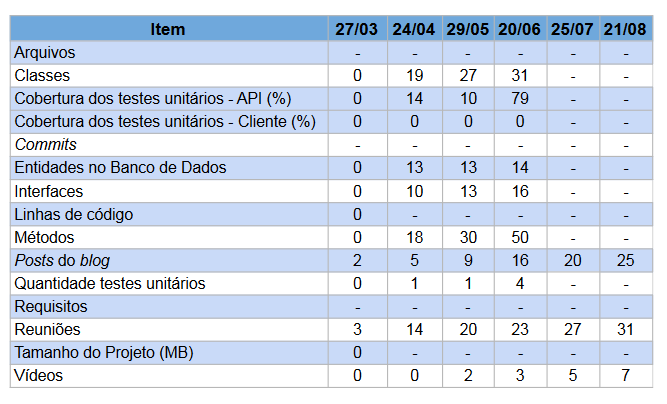
\includegraphics[width=1.0\textwidth]{anexos/Imagens_PesquisaAceitacao/Metricas.png}
% \fonte{Os autores}
% \end{figure}
% \FloatBarrier
% ------------------------------------------------------------
\section{Plano de testes}
%--------------------------------------------------------------
Segundo \citeonline{Polo:2020}, por definição, os testes de \textit{software} visam assegurar que um sistema/programa atenda às necessidades dos seus usuários, assim como também permitem descobrir defeitos no funcionamento antes de disponibilizá-lo para uso. Na realização dos testes, segundo \citeonline{SOMMERVILLE:2019}, são usados dados artificiais para a sua execução.

\begin{citacao}
Os resultados dos testes são verificados para descoberta de erros, anomalias ou informações não funcionais sobre a sua execução, por exemplo, análise de desempenho, utilização de memória etc \cite{Polo:2020}.
\end{citacao}

Considerando os apontamentos dos autores, e de modo a garantir um bom funcionamento do sistema \gls{ifriends} além de prevenir eventuais erros, foi planejado a realização de testes considerados necessários. Dessa forma, esta seção visa apresentar os testes aplicados no sistema \gls{ifriends}.

%--------------------------------------------------------------
\subsection{Testes unitários}
%--------------------------------------------------------------
Segundo \citeonline{SOMMERVILLE:2011}, por testes unitários se compreende o processo de testar componentes de programa, sendo eles métodos ou classes de objeto. Funções individuais ou métodos são os tipos mais simples de unidades. Seus testes devem ser chamados de para essas rotinas sob diferentes parâmetros. O autor ainda complementa dizendo: 

\begin{citacao}
Quando você está testando as classes de objeto, deve projetar os testes para fornecer uma cobertura de todas as características do objeto. Isso significa que você deve: testar todas as operações associadas ao objeto, definir e verificar o valor de todos os atributos associados ao objeto e colocar o objeto em todos os estados possíveis, o que significa simular todos os eventos que causam mudanças de estado
\cite{SOMMERVILLE:2011}.
\end{citacao}

Dessa forma, para o sistema \gls{ifriends}, cada novo método será feito pensando na criação dos testes unitários, de modo a também facilitar, posteriormente, seu planejamento. Os testes serão construídos efetivamente sempre após a criação de seus respectivos métodos ou classes, ou seja, após criar um método de cadastrar pergunta será feito o teste para verificar se todas as funcionalidades estão implementadas corretamente.

Além disso, considerando os apontamentos realizadas por \citeonline{StefanBechtold2021Apr} foi escolhido o \gls{JUnit} 5 como facilitador para execução dos testes automatizados na linguagem Java. Segundo a documentação do \gls{JUnit}, o \gls{framework} possui vários métodos para facilitar a verificação dos resultados, eles fazem parte da classe \textit{Assertions}, e funcionam através de anotações ``@Test'' para dizer ao sistema que o que está abaixo da anotação é um método ou uma classe de teste. O escopo sempre possui três divisões, sendo elas: cenário, que visa a preparação dos dados a serem testados; ação, que se refere ao que o teste deve executar, e a verificação, para conferir se o teste foi realizado conforme planejado.

A \autoref{exemplo teste} é um exemplo da estrutura de um teste, sendo este criado para o testar o método de salvar um usuário no banco de dados:

\begin{figure}[htb]
\centering
\caption{\label{exemplo teste} Teste na API}
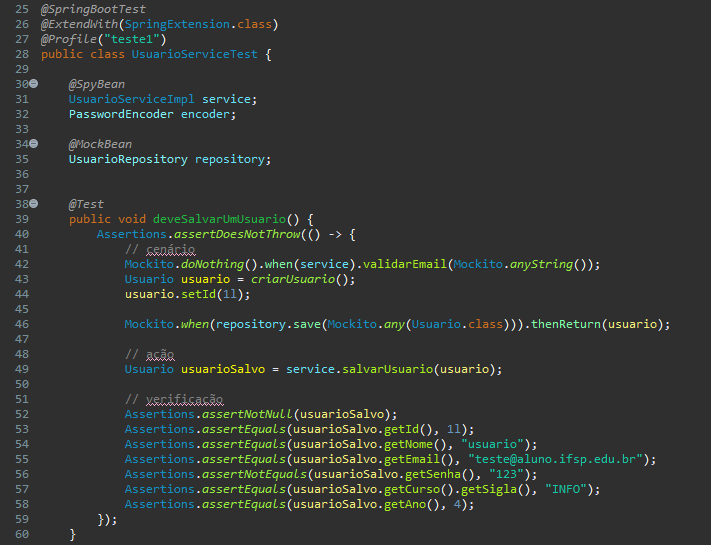
\includegraphics[width=1\textwidth]{anexos/Imagens_Testes/API_teste.png}
\fonte{Os autores}
\end{figure}
\FloatBarrier

Conforme mostrado na \autoref{exemplo teste}, é possível visualizar as anotações ``@SpyBean'' e ``@MockBean'', eles são responsáveis por dizer ao \gls{SpringBoot} quais classes ele deve gerenciar e trazer para dentro do seu próprio contexto. Com a anotação ``@Profile'' é possível definir qual arquivo de propriedades será utilizado, no caso da \autoref{exemplo teste} é o arquivo que contém as configurações para o banco de dados teste.

Já para a cobertura de testes unitários está sendo utilizado o \acs{jacoco}. De acordo com sua documentação, a tecnologia oferece recursos integráveis com o \gls{JUnit}, e o \gls{Eclipse}, \acs{ide} utilizada para construção da \acs{api}. A \autoref{grafico de testes} mostra o gráfico de cobertura de testes, realizado para a classe serviço de pergunta do \gls{ifriends}:

\begin{figure}[htb]
\centering
\caption{\label{grafico de testes} Cobertura de testes}
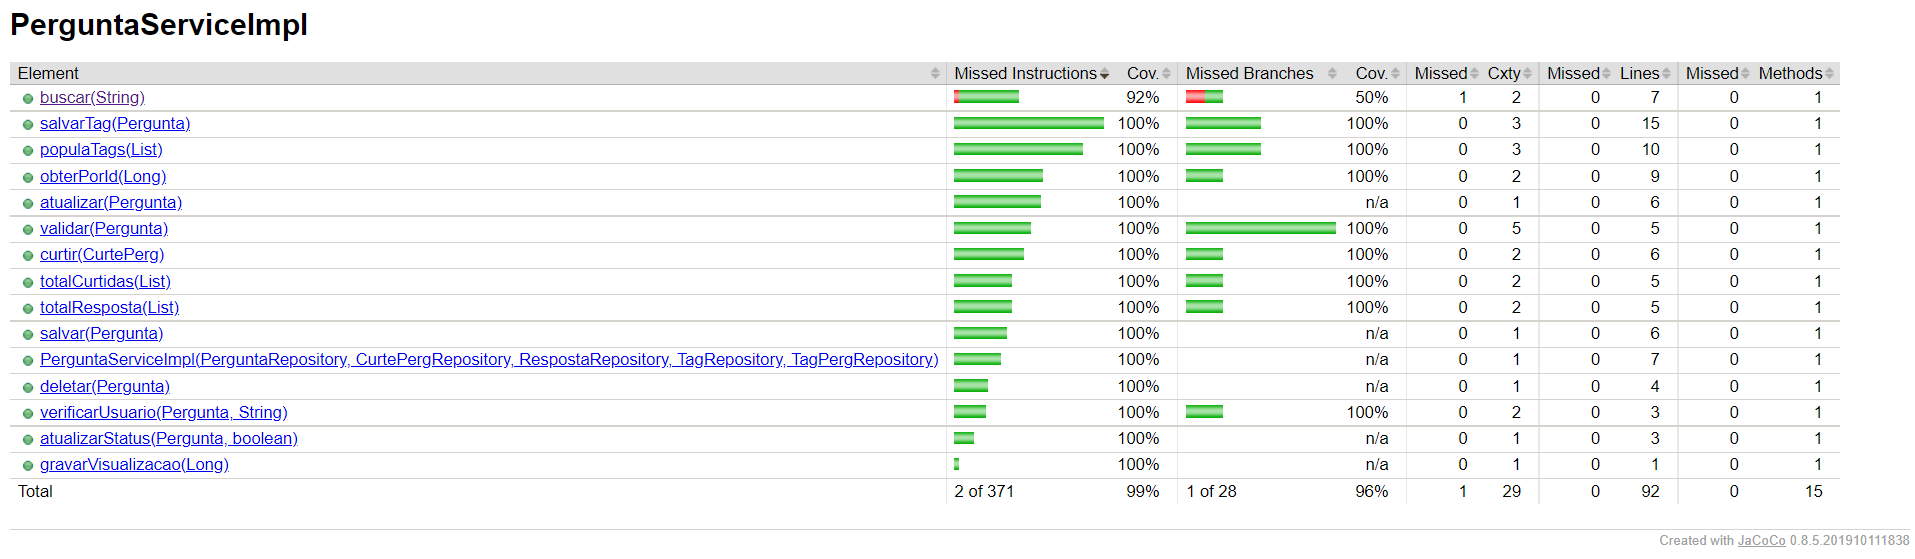
\includegraphics[width=1\textwidth]{anexos/Imagens_Testes/API_grafico-testes.png}
\fonte{Os autores}
\end{figure}
\FloatBarrier

Após a observação feita do gráfico na \autoref{grafico de testes}, a primeira coluna possui os nomes de todos os métodos da classe; a segunda coluna é possível saber a porcentagem total do percurso testado de cada método; a terceira coluna mostra a porcentagem de todas as operações básicas testadas, e o restante das colunas mostram, respectivamente, a quantidade de operações, linhas e métodos da classe.

%--------------------------------------------------------------
\subsection{Testes de usabilidade}
%--------------------------------------------------------------
Segundo \citeonline{alura2022}, testes de usabilidade é uma técnica de caixa-preta qual visa o mapeamento da interação de usuários com o produto de modo a descobrir problemas e pontos de melhorias. 

Na parte de usabilidade, a equipe definiu que, primeiramente, será validada a interface de usuário, verificando se o sistema segue uma coerência baseada nas 10 heurísticas de Nielsen e nos requisitos de acessibilidade especificados no W3C, ou seja, será um teste feito inicialmente pelos próprios desenvolvedores e conforme a frequência de entregas. Ainda para a interface, conforme os requisitos da disciplina,  o sistema deve ser inserido em um validador de interfaces que será especificado nesta documentação, com seus resultados, após a última entrega - quando finalizados todos os testes com usuários.

%----------------------------------------------------------------
\subsubsection{Cenário de testes}
%----------------------------------------------------------------
Segundo \citeonline{Polo:2020}, um cenário é uma história que descreve a maneira pela qual o sistema pode ser usado, esses cenários devem ser realistas e devem ser testados por usuários reais. Ainda, como características fundamentais, o autor \citeonline{Polo:2020} destaca uma narrativa mais próxima possível da realidade de utilização do sistema, além de ser um cenário de fácil avaliação. 

Dessa forma, para o cenário de teste do projeto \gls{ifriends} serão recrutados estudantes do próprio \acs{ifsp} de forma aleatória, e por meio de uma pesquisa presencial a equipe de \textit{design} deverá cobrir as seguintes etapas: 

\begin{itemize}
%---
    \item \textbf{Introdução amigável:} uma boa introdução, ainda mais sendo ela amigável, deixará o \gls{friend} mais confortável e mais preparado para seguir com a pesquisa. Dessa forma, realizar uma breve introdução informando o motivo da sua presença, qual é a finalidade da pesquisa e informar previamente as ações ele irá realizar é fundamental;
%---    
    \item \textbf{Perguntas relacionadas:} como os entrevistados serão os próprios alunos do \acs{ifsp}, esta etapa não será muito complexa. Após realizar a introdução amigável, a equipe de \textit{design} deverá desencadear uma conversa inicial a respeito do assunto que aquela dinâmica deverá seguir, como, por exemplo, realizar perguntas que se relacionem com o projeto ou com sua problemática; 
%---
    \item \textbf{Apresentação da solução:} após envolver o \gls{friend} no assunto, a próxima etapa é mostrar a aplicação, fornecer a possibilidade de ele interagir de fato com o sistema. Se tratando de sua primeira interação, logo de início o \gls{friend} mostrará um certo comportamento, portanto é fundamental que a equipe de \textit{design} identifique essa ``resposta emocional'';
%---
    \item \textbf{Propor desafios:} a próxima etapa da pesquisa é propor desafios para que o \gls{friend} realize na entrevista, dentro desses desafios é importante testar os principais fluxos do sistema. Após concluir todos os desafios planejados, a equipe de \textit{design} pode fazer algumas perguntas sobre a experiência, desempenho e precisão; 
%---
    \item \textbf{\textit{Feedback} geral:} por fim, a última da etapa da entrevista refere-se a receber um \textit{feedback} geral por parte do \gls{friend} assim como dar os devidos agradecimentos por sua participação e disposição;
%---
\end{itemize}

Após cobrir os requisitos acima citados, a equipe irá aplicar a pesquisa de satisfação geral criada com base na metodologia de satisfação de clientes, a chamada \acs{nps}, para entender melhor o quão satisfeitos os usuários estão com sistema e como podemos melhorá-lo, disponível de forma digital em \href{https://t.maze.co/124107555}{https://t.maze.co/124107555}, podendo ser difundida entre os usuários ou anexada ao próprio sistema livremente, sem a necessidade de passar por uma nova entrevista.

Vale ressaltar que no \autoref{script_entrevista} podem ser encontrados mais detalhes a respeito da pesquisa. E no \autoref{resultado_entrevista} os resultados, apontamentos e considerações desta etapa. 
